\newcommand{\Titolo}{Verbale interno 01}
\newcommand{\Gruppo}{SWEnergy}
\newcommand{\Data}{17/10/2023}
\newcommand{\Mail}{\href{mailto:project.swenergy@gmail.com}{project.swenergy@gmail.com}}
\newcommand{\Versione}{0.1.0}
\newcommand{\Descrizione}{Primo incontro, nome, logo e metodi di comunicazione}

\newcommand{\copertina}{
	\begin{titlepage}
		\begin{center}
			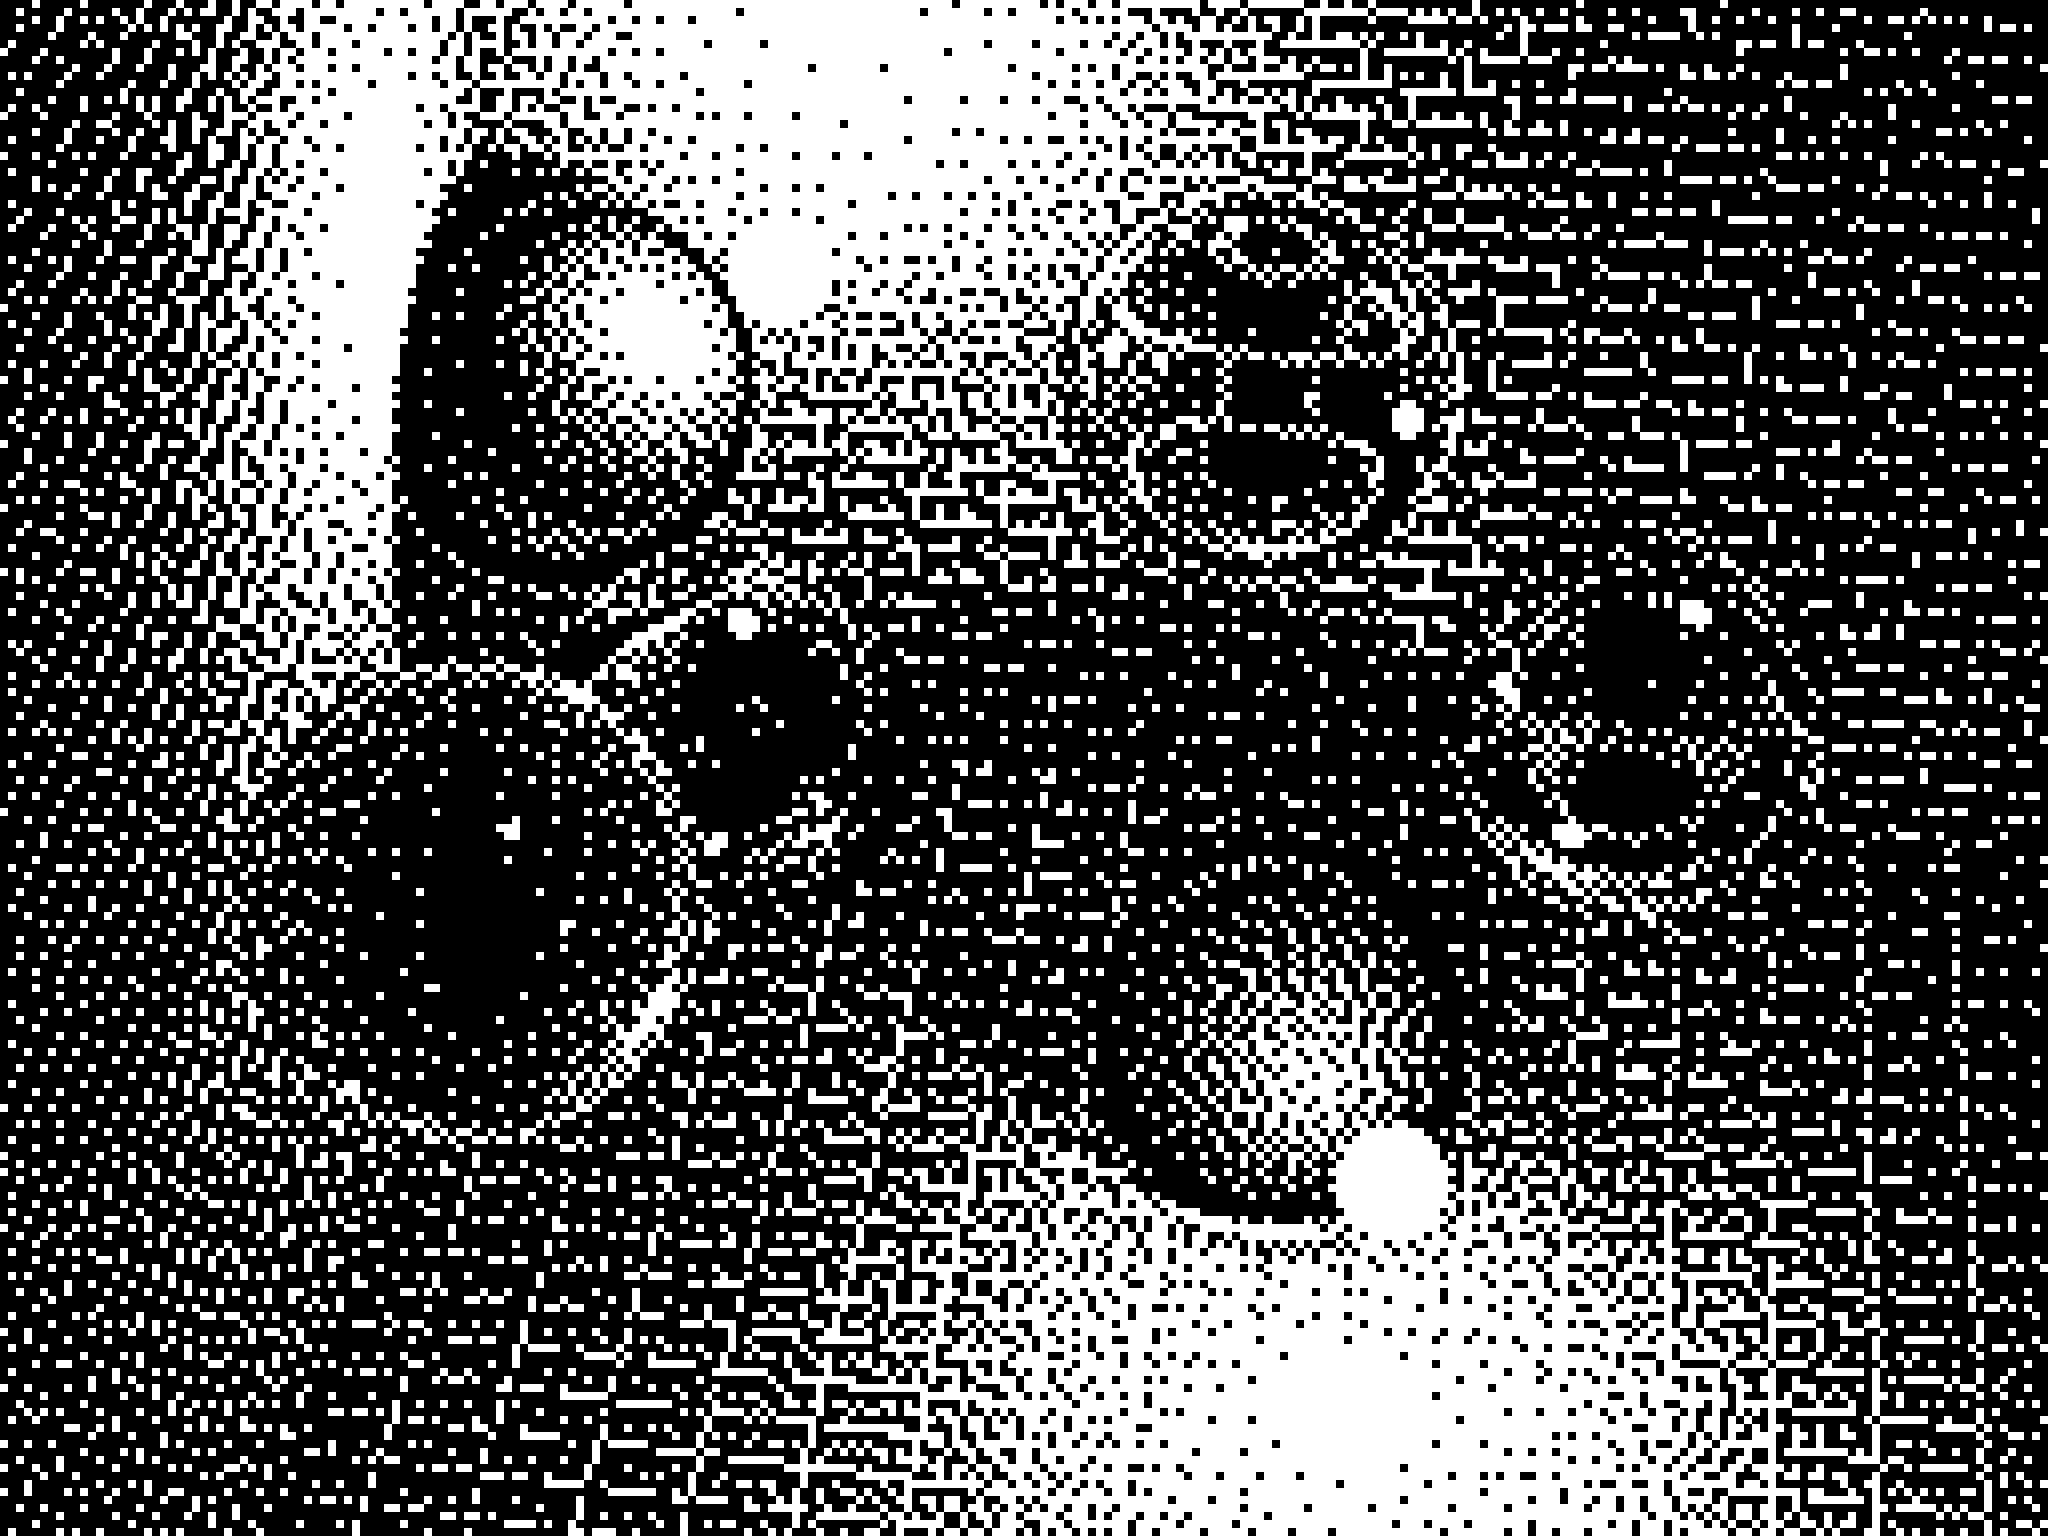
\includegraphics[width=0.5\textwidth]{img/logo}	\\
			\vspace{1cm}
			\Mail{}	\\
			\vspace{0.5cm}
			\textbf{\begin{large} \Titolo{} \end{large}}	\\
			\vspace{1cm}
			\textbf{Descrizione:} \Descrizione{} \\
			\vspace{1cm}
		\end{center}
		\begin{center}
			\begin{tabular}{lll}
				\textbf{Stato} 			& Non approvato	&	\\ 
				\textbf{Data}			& \Data{}	&	\\
				\midrule
				\textbf{Redattori} 		& Alessandro Tigani Sava 	&	\\  
				\textbf{Verificatori} 	&	&	\\
				\textbf{Approvatori} 	&	&  	\\    
				\midrule
				\textbf{Versione}		& \Versione{}	& 	\\
			   \end{tabular}
		\end{center}
		\vspace{5cm}
		\begin{flushright}
			\begin{tabular}{ll}
				Il responsabile:	&  	Nuvolaris	\\
									&				\\
									&	\underline{\hspace{3cm}} 	\\
			\end{tabular}
		\end{flushright}
	\end{titlepage}
}

\fancypagestyle{plain}{
  	\fancyhf{}
  	\rhead{ 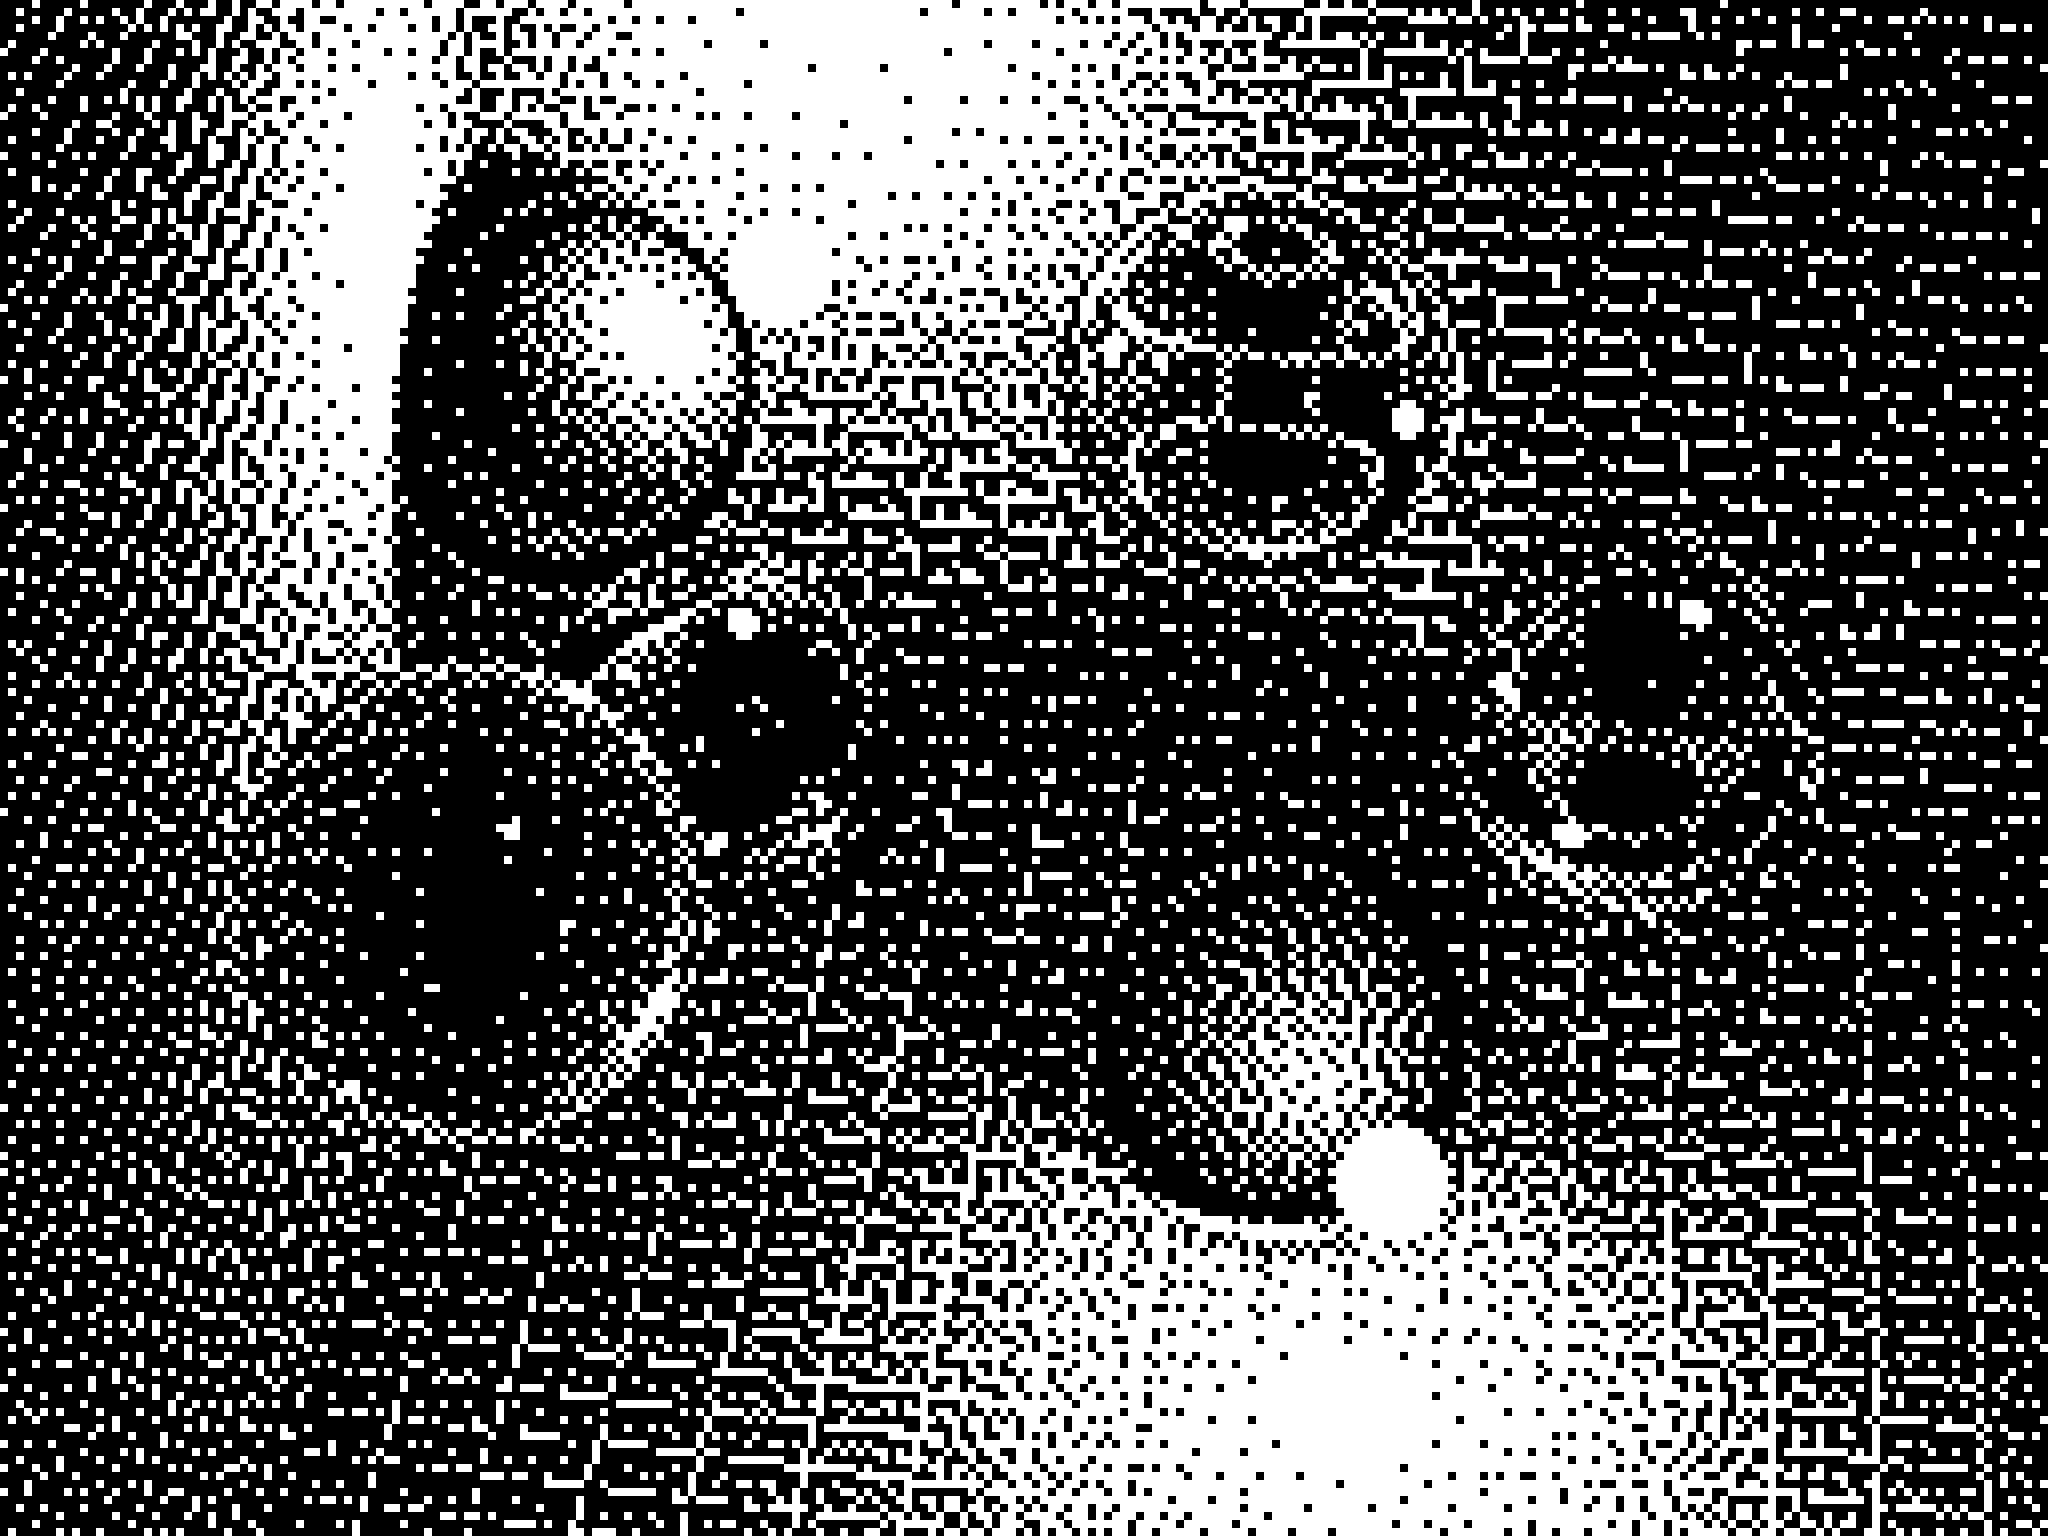
\includegraphics[scale=0.02]{img/logo.png}}
  	\lhead{\Gruppo}
  	\lfoot{\Titolo{}}
  	\rfoot{\thepage{}} 
  	\renewcommand{\headrulewidth}{0.2pt}
  	\renewcommand{\footrulewidth}{0.2pt}
}
\pagestyle{plain}